\documentclass{beamer}
\graphicspath{{../graphics/}}
\usepackage{listings}
\usepackage{ulem}
\usepackage{subcaption}
\usepackage{algorithm2e}

\mode<presentation>
{
  \usetheme{Darmstadt}
  \setbeamertemplate{footline}[frame number]
  \setbeamercovered{navigation symbols}
  \setbeamercovered{transparent}
}

\AtBeginSection[]
{
   \begin{frame}
        \frametitle{Table of Contents}
        \tableofcontents[sectionstyle=show/hide,subsectionstyle=show/show/hide]
   \end{frame}
}

%\usepackage[danish]{babel}
\usepackage[T1]{fontenc}

\usepackage[utf8]{inputenc}

\usepackage{times}

\usepackage{tikz}

\usepackage{subfigure}

\title[Mapping med Lego-robot]{Mapping med Lego-robot}

\subtitle{SW505E13}

\author[SW505E13]{Mikkel Sand\o ~Larsen, \and Bruno Thalmann, \and Stefan Marstrand Getreuer Micheelsen, \and Stefan Thilemann, \and Mikael Elki\ae r Christensen, \and Anders R. Nielsen}

\institute[Aalborg University]
{
  Department of Computer Science\\
  Aalborg University}

\date[CFP 2003]{31. Januar 2014}

\begin{document}

%--------------------------------------------------
%     INTRODUKTION
%--------------------------------------------------

\begin{frame}
  \titlepage
\end{frame}

\begin{frame}
    \frametitle{Table of Contents}
    \tableofcontents[sectionstyle=show/show,subsectionstyle=hide/hide/hide]
\end{frame}

\section{Introduction}

%--------------------------------------------------
%     BAGGRUND
%--------------------------------------------------
\subsection{Baggrund}
\begin{frame}[fragile]{Anvendelse}
	Stort anvendelsesområde for robotter
	\begin{itemize}
		\item Industri
			\begin{itemize}
			\item Droner (overvågning/kortlægning)
			\item Lager robotter
			\end{itemize}
		\item Privat
			\begin{itemize}
			\item Støvsuger robotter
			\item Plæneklipper robotter
		\end{itemize}
	\end{itemize}
\end{frame}

\begin{frame}[fragile]{Grundlæggende problemstillinger}
	\begin{columns}
		\begin{column}{0.5\textwidth}
			Krav til robotten så den kan begå sig i dens omgivelser
			\linespace
			\begin{itemize}
				\item Lokation (interaktion med omgivelser)
				\item En form for kort (til navigation)
			\end{itemize}
		\end{column}
		\pause
		\begin{column}{0.5\textwidth}
			SLAM (\textbf{S}imultaneous \textbf{L}ocalization \textbf{A}nd \textbf{M}apping)
			\linespace
			\begin{itemize}
				\item \textit{Svært!}
					\begin{itemize}
						\item Approximering af lokation
					\end{itemize}
				\item Lokation afhængig af kort, og omvendt
			\end{itemize}
		\end{column}
\end{columns}
\end{frame}


\subsection{Problem}
%--------------------------------------------------
%     AFGRÆNSNING
%--------------------------------------------------
\begin{frame}[fragile]{Afgrænsning}
	\begin{itemize}
		\item Lokalisering vha. color-tracking fra Kinect
	\end{itemize}
	
	\linespace
	\pause
	
	Simplificering af robottens kørselsmiljø:
	\begin{itemize}
		\item Robottens verden er 90 grader
		\item Verdenen er et afgrænset område
		\item Verdenen er plan og befinder sig indendørs
	\end{itemize}
	\linespace
	Mindsker kravene til robotten og gør det nemmere at evaluere resultater.
\end{frame}

%--------------------------------------------------
%     PROBLEMFORMULERING
%--------------------------------------------------
\begin{frame}[fragile]{Problemformulering}
	\begin{center}
		\textit{Hvordan kan der konstrueres software til en robot, hvis formål er at kortlægge en ukendt verden, forudsat at den til enhver tid kender sin position?}
	\end{center}
\end{frame}

%--------------------------------------------------
%     MÅLSÆTNING
%--------------------------------------------------
\begin{frame}[fragile]{Målsætning}
	Grundlag for evaluering af det endelige produkt:
	\begin{itemize}
	\item To forskellige overvejelser
		\begin{itemize}
			\item Hastighed af kortlægning
			\item Præcision af kortlægning
		\end{itemize}
	\end{itemize}
	\linespace
	\pause
	
	Målet med dette projekt:
	\begin{itemize}
		\item At bygge en robot, der kan konstruere et præcist kort
	\end{itemize}
	\linespace
	\pause
	
	Vurdering af valgte målsætning:
	\begin{itemize}
		\item \textit{Det skal være muligt at navigere alene ud fra informationen i kortet og køre fra et hjørne til det diagonalt modsatte}
	\end{itemize}
\end{frame}

%--------------------------------------------------
%     FORSØGSOPSTILLING
%--------------------------------------------------
\subsection{Forsøgsopstilling}
\begin{frame}[fragile]{Kørselsmiljø set fra siden}
	\begin{figure}
		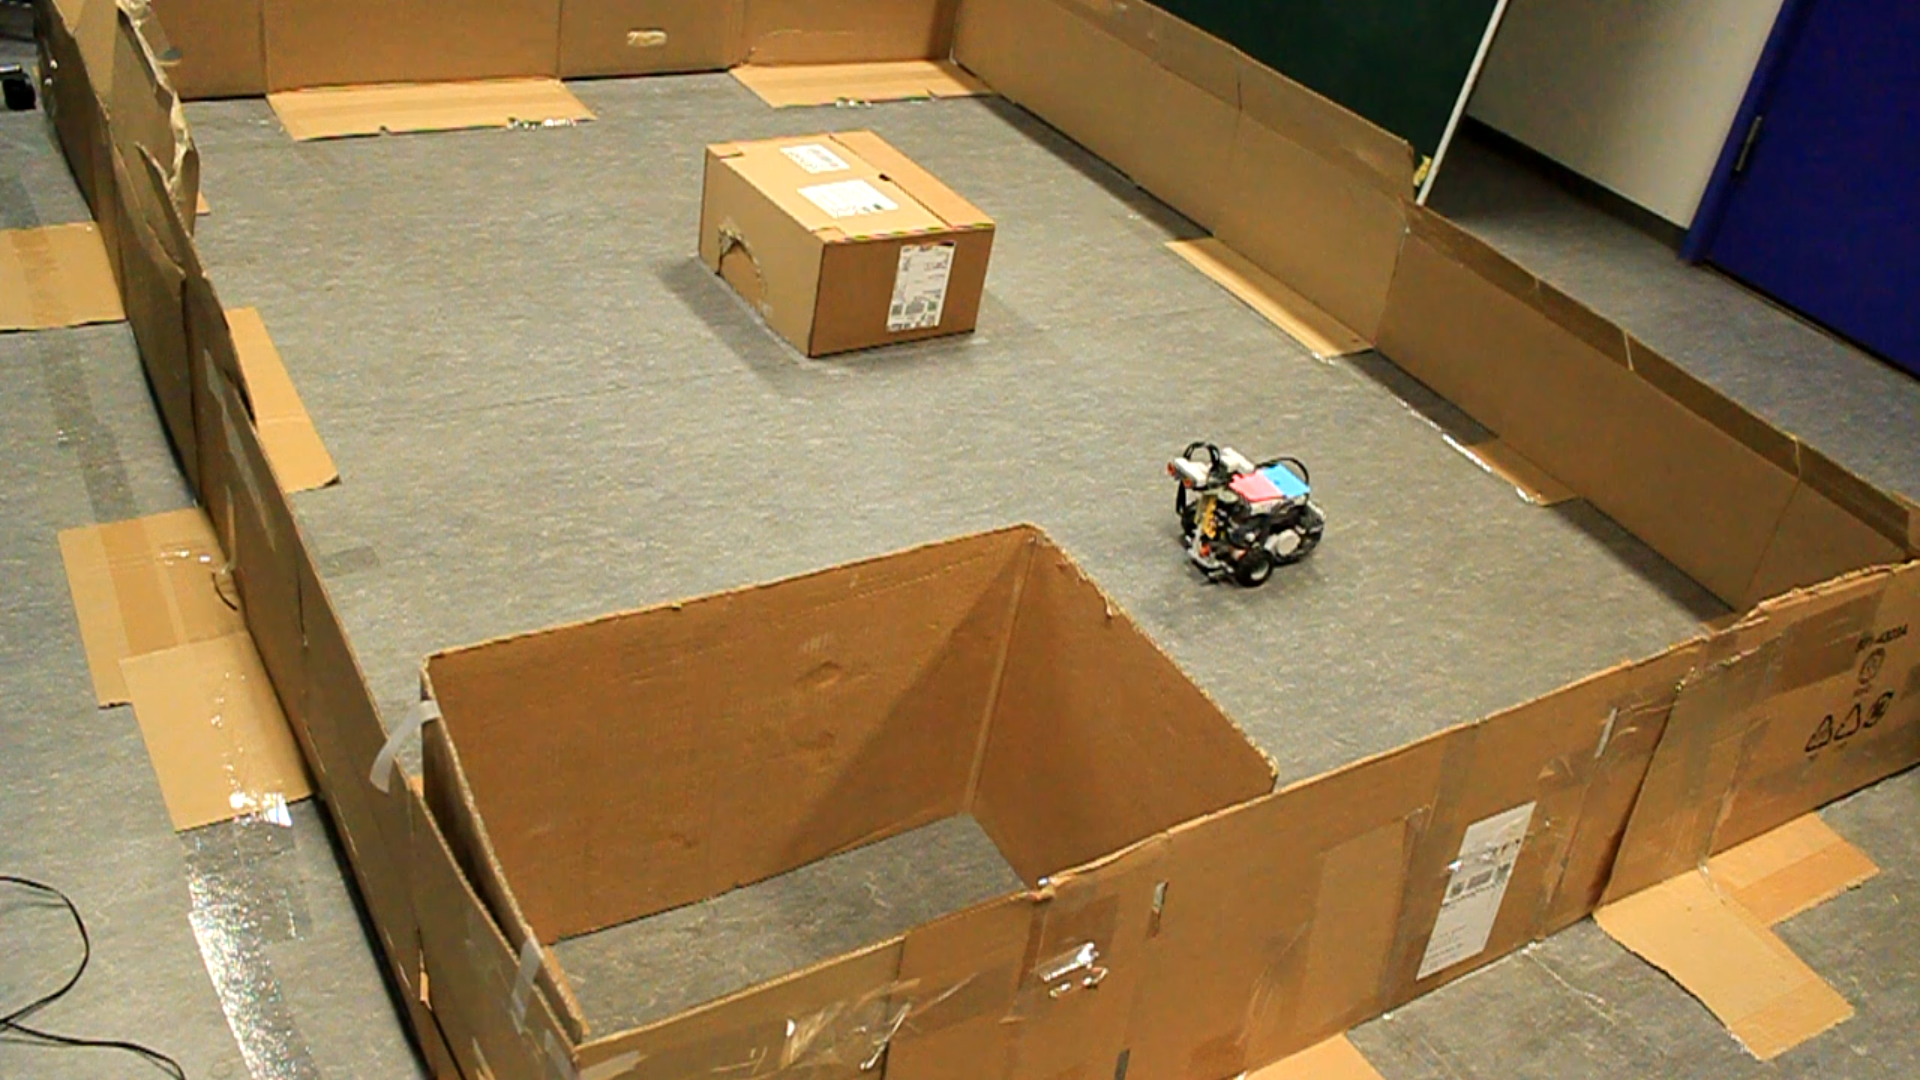
\includegraphics[width=1\textwidth]{verden/opstilling.png}
	\end{figure}
\end{frame}

\begin{frame}[fragile]{Forsøgsopstilling og Kinect}
	\begin{columns}
		\begin{column}{0.5\textwidth}
			\begin{itemize}
				\item Kørselsmiljø set fra Kinect
			\end{itemize}
			\begin{figure}
				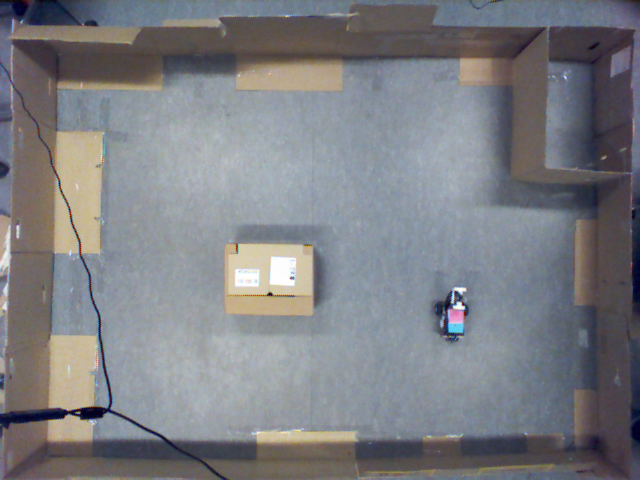
\includegraphics[width=1\textwidth]{evaluering/emptyGrid.png}
			\end{figure}
		\end{column}
		
		\begin{column}{0.5\textwidth}
				\begin{itemize}
					\item Montering af Kinect i loft
				\end{itemize}
			\begin{figure}
				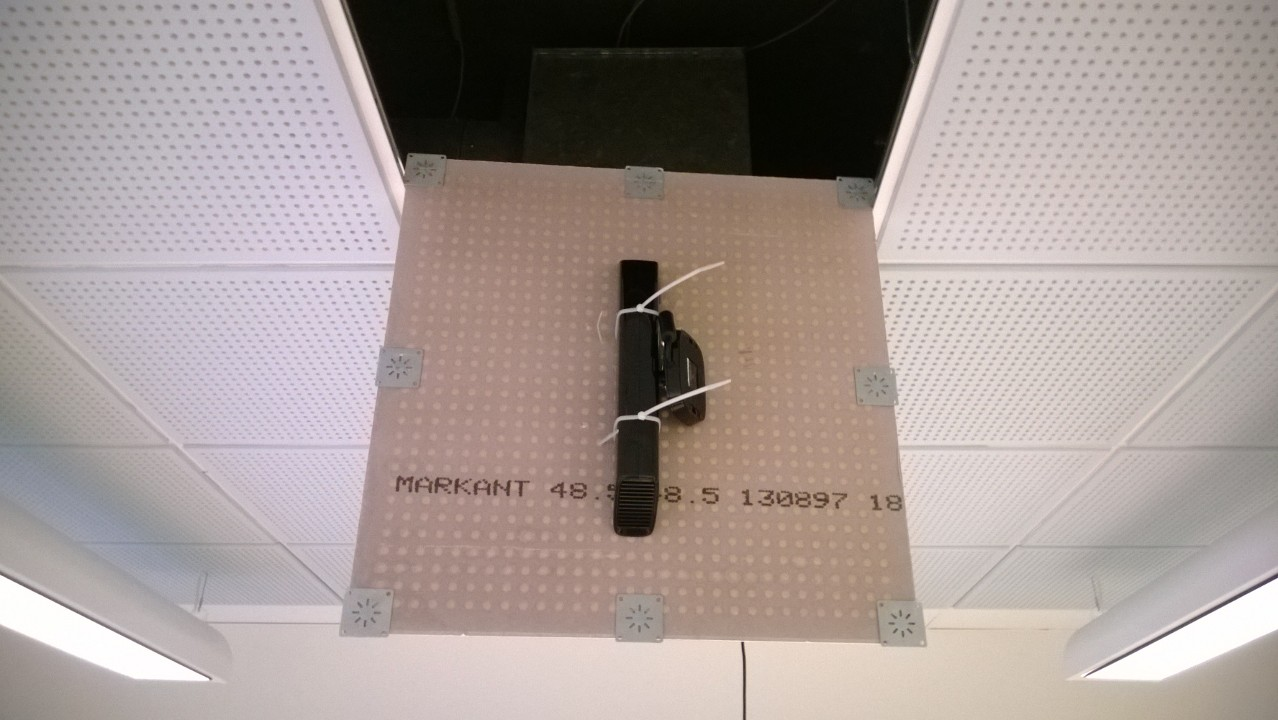
\includegraphics[width=1\textwidth]{verden/kinect.jpg}
			\end{figure}
	\end{column}
\end{columns}
\end{frame}

%--------------------------------------------------
%     EVALUERINGSMETODE
%--------------------------------------------------
\subsection{Evaluering af målsætning}
\begin{frame}[fragile]{Vurderingsmål}
	\begin{itemize}
		\item Approximering af et optimalt kort for forsøgsopstillingen
	\end{itemize}
	
	\begin{figure}
		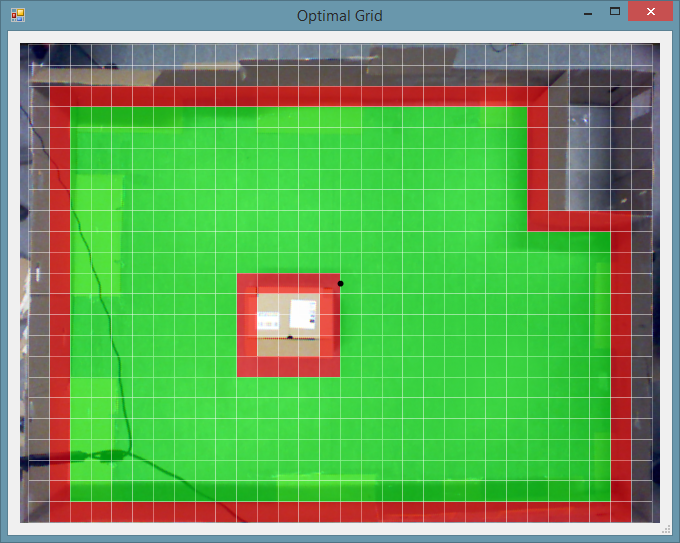
\includegraphics[width=.65\textwidth]{evaluering/optimalgrid.png}
	\end{figure}
\end{frame}
\section{Teori}
\subsection{Grundlæggende}
\begin{frame}{Occupancy Grid}
\begin{figure}[h] % Kørselsmiljø og et occupancy grid
\centering
	\begin{subfigure}[b]{.48\textwidth}
	\centering
	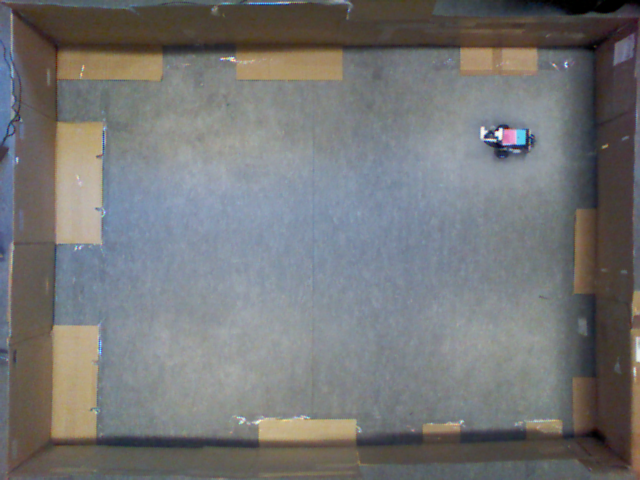
\includegraphics[width=\textwidth]{verden/oppefra_m_walle}
	\caption{Aktuelt Kørselsmiljø.}
	\label{map:world}
	\end{subfigure}
	\hfill
	\begin{subfigure}[b]{.48\textwidth}
	\centering
	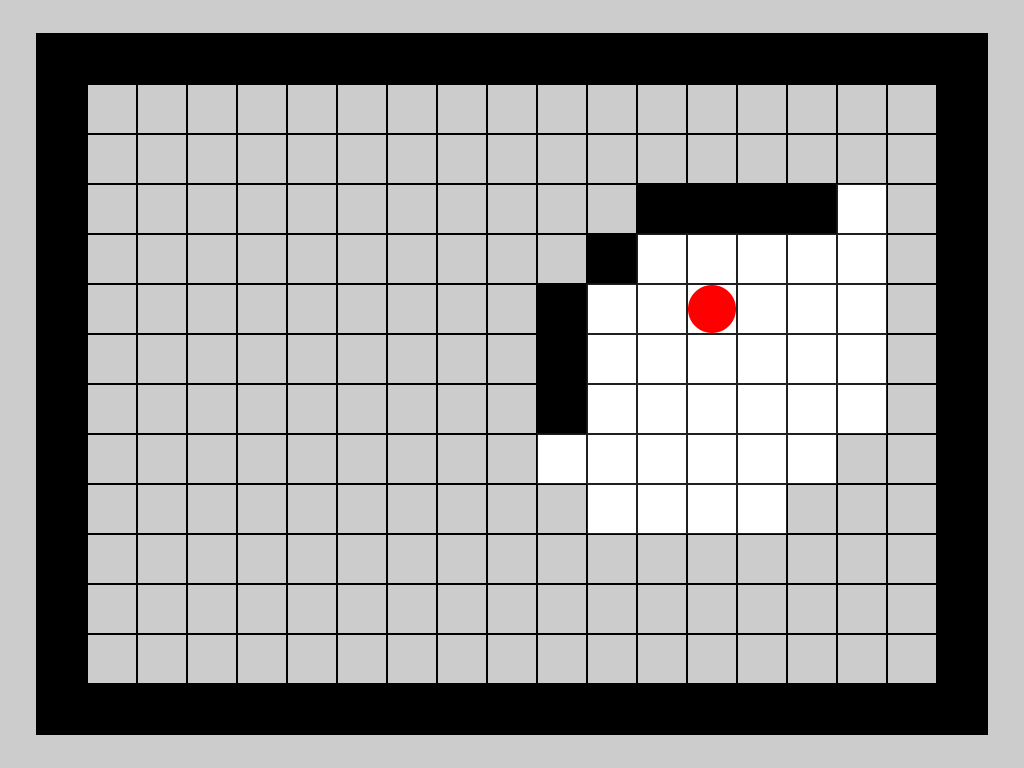
\includegraphics[width=\textwidth]{verden/occupancy_grid_verden}
	\caption{Occupancy Grid.}
	\label{map:occupancy_grid}
	\end{subfigure}

\end{figure}
\end{frame}
\begin{frame}{Bayes Regel}
Opdatering af troen på en proposition ved ny evidens
\[
\begin{split}
P(h \mid e) = \frac{P(e \mid h) \times P(h)}{P(e)}
\end{split}
\]
\end{frame}

\begin{frame}{Log Odds}
\begin{figure}
\centering 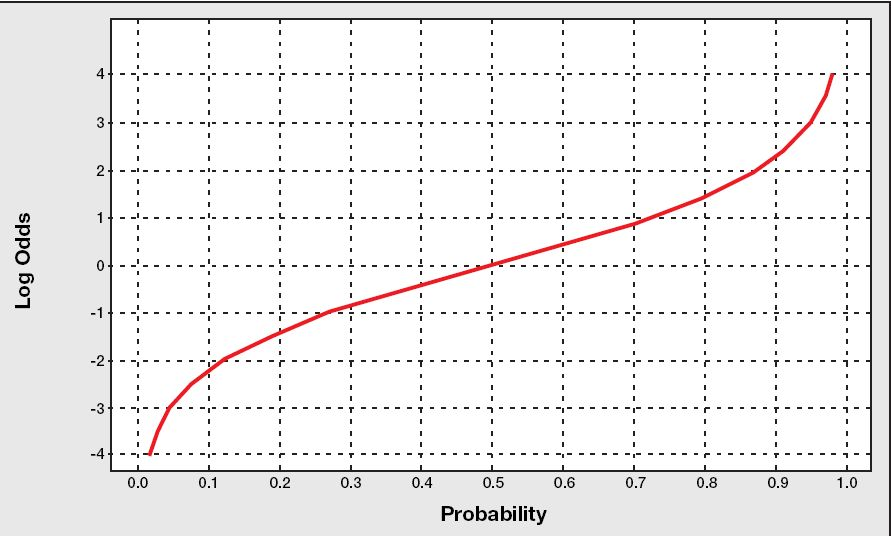
\includegraphics[scale=.2]{LogOdds}
\label{logoddsimg}
\end{figure}

%Log odds er en metode der kan benyttes for at undgå, at komponenterne i Bayes Regel enten bliver definitivt sande eller falske.
%
%Der kan derfor indføres en funktion, \textit{log odds ratio}, som mapper sandsynlighedsværdierne fra $[0;1]$ til $[-\infty;\infty]$.
%Oddset for tilstand $x$ er defineret som forholdet mellem sandsynlighederne for $x$ og $\lnot x$: 

\begin{tabular}{ p{0.5\linewidth} p{0.5\linewidth} }
$ l(x) = \log \frac{p(x)}{1 - p(x)} $ & 
$ bel_t(x) = 1 - \frac{1}{1 + exp\{l_x\}}\label{logodds:bel} $
\end{tabular}
\end{frame}

\subsection{Occupancy Grid}

\begin{frame}{Binært Bayes Filter}
Kan bruges når verdenens tilstand er statisk

\begin{algorithm}[H]
\textbf{BinaryBayesFilter($l_{t-1}, z_t$)} \\
\Indp $l_t = l_{t-1} + \log \frac{p(x \mid z_t)}{1-p(x \mid z_t)} - \log \frac{p(x)}{1-p(x)}$ \\
\Return{$l_t$}
\end{algorithm}
\end{frame}

\begin{frame}{Occupancy grid}
\begin{algorithm}[H]
OccupancyGridMapping(\{$l_{t-1,i}$\}, $x_t$, $z_t$):

\ForAll{cells $ m_i $}
{
\eIf{$ m_i $ is in the perceptual field of $ x_t $}
%then
{ $ l_{t,i} = l_{t-1,i} $ + \textbf{inverse\_sensor\_model} $( m_i, x_t, z_t ) - l_0$\\ }
%else
{ $ l_{t,i} = l_{t-1,i}  $\\ }
}
\Return {$ \{l_{t,i}\} $}
\end{algorithm}
\end{frame}

\begin{frame}{Occupancy grid}
\begin{algorithm}[H]
OccupancyGridMapping(\{$l_{t-1,i}$\}, $x_t$, $z_t$):

\ForAll{cells $ m_i $}
{
\eIf{$ x_i = x_r$ or $y_i = y_r$}
%then
{ $ l_{t,i} = l_{t-1,i} $ + \textbf{inverse\_sensor\_model} $( m_i, x_t, z_t ) - l_0$\\ }
%else
{ $ l_{t,i} = l_{t-1,i}  $\\ }
}
\Return {$ \{l_{t,i}\} $}
\end{algorithm}
\end{frame}

\subsection{Sensormodeller}
\begin{frame}{Simpel sensormodel}

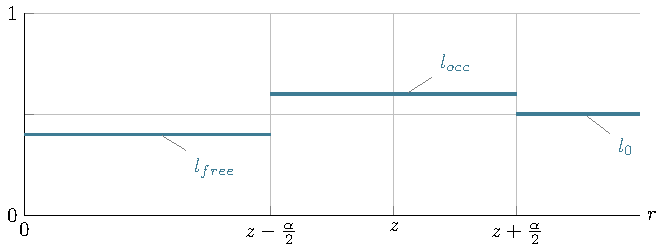
\includegraphics{simple_sensormodel.pdf}
\end{frame}

\begin{frame}{Gaussisk sensormodel}

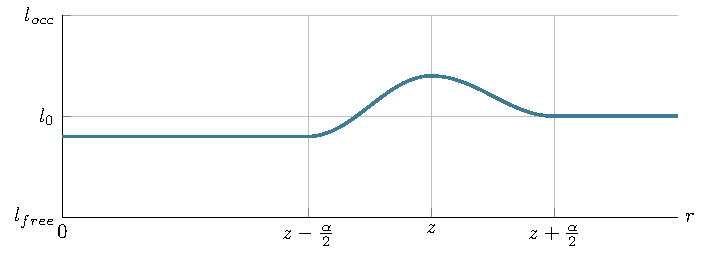
\includegraphics{gaussian_sensormodel.pdf}
\end{frame}

\begin{frame}{Sammenligning af sensormodeller}
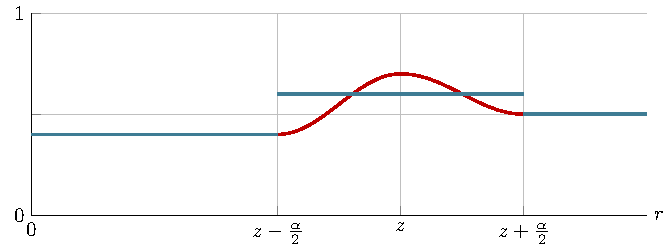
\includegraphics{combined_sensormodel}
\end{frame}



%Robottens design
\section{Robottens design}
\subsection{Præsentation af designet}
\begin{frame}
\frametitle{Overordnet}
\begin{center}
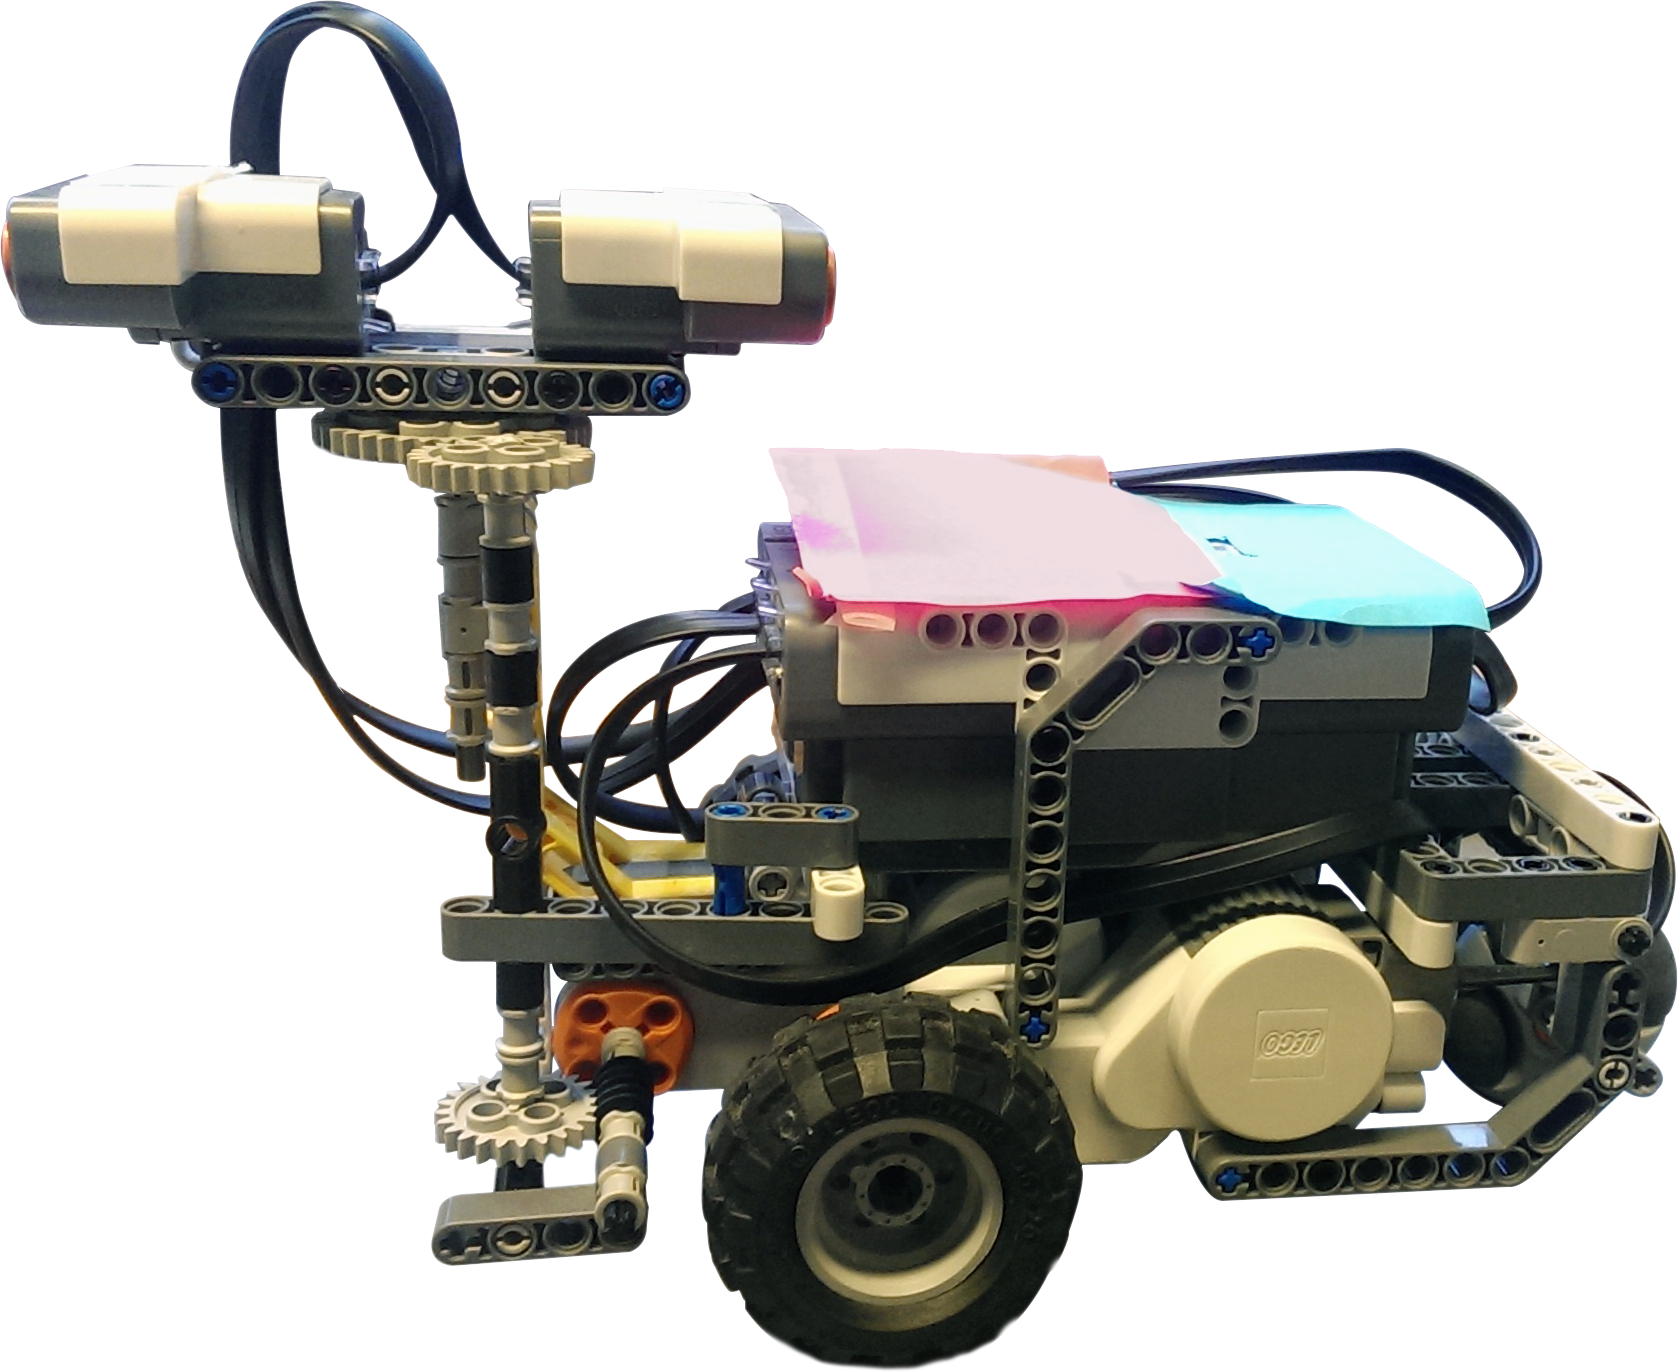
\includegraphics[scale=0.15]{whalle}
\end{center}
\end{frame}

\begin{frame}
\frametitle{Gearing}
\begin{center}
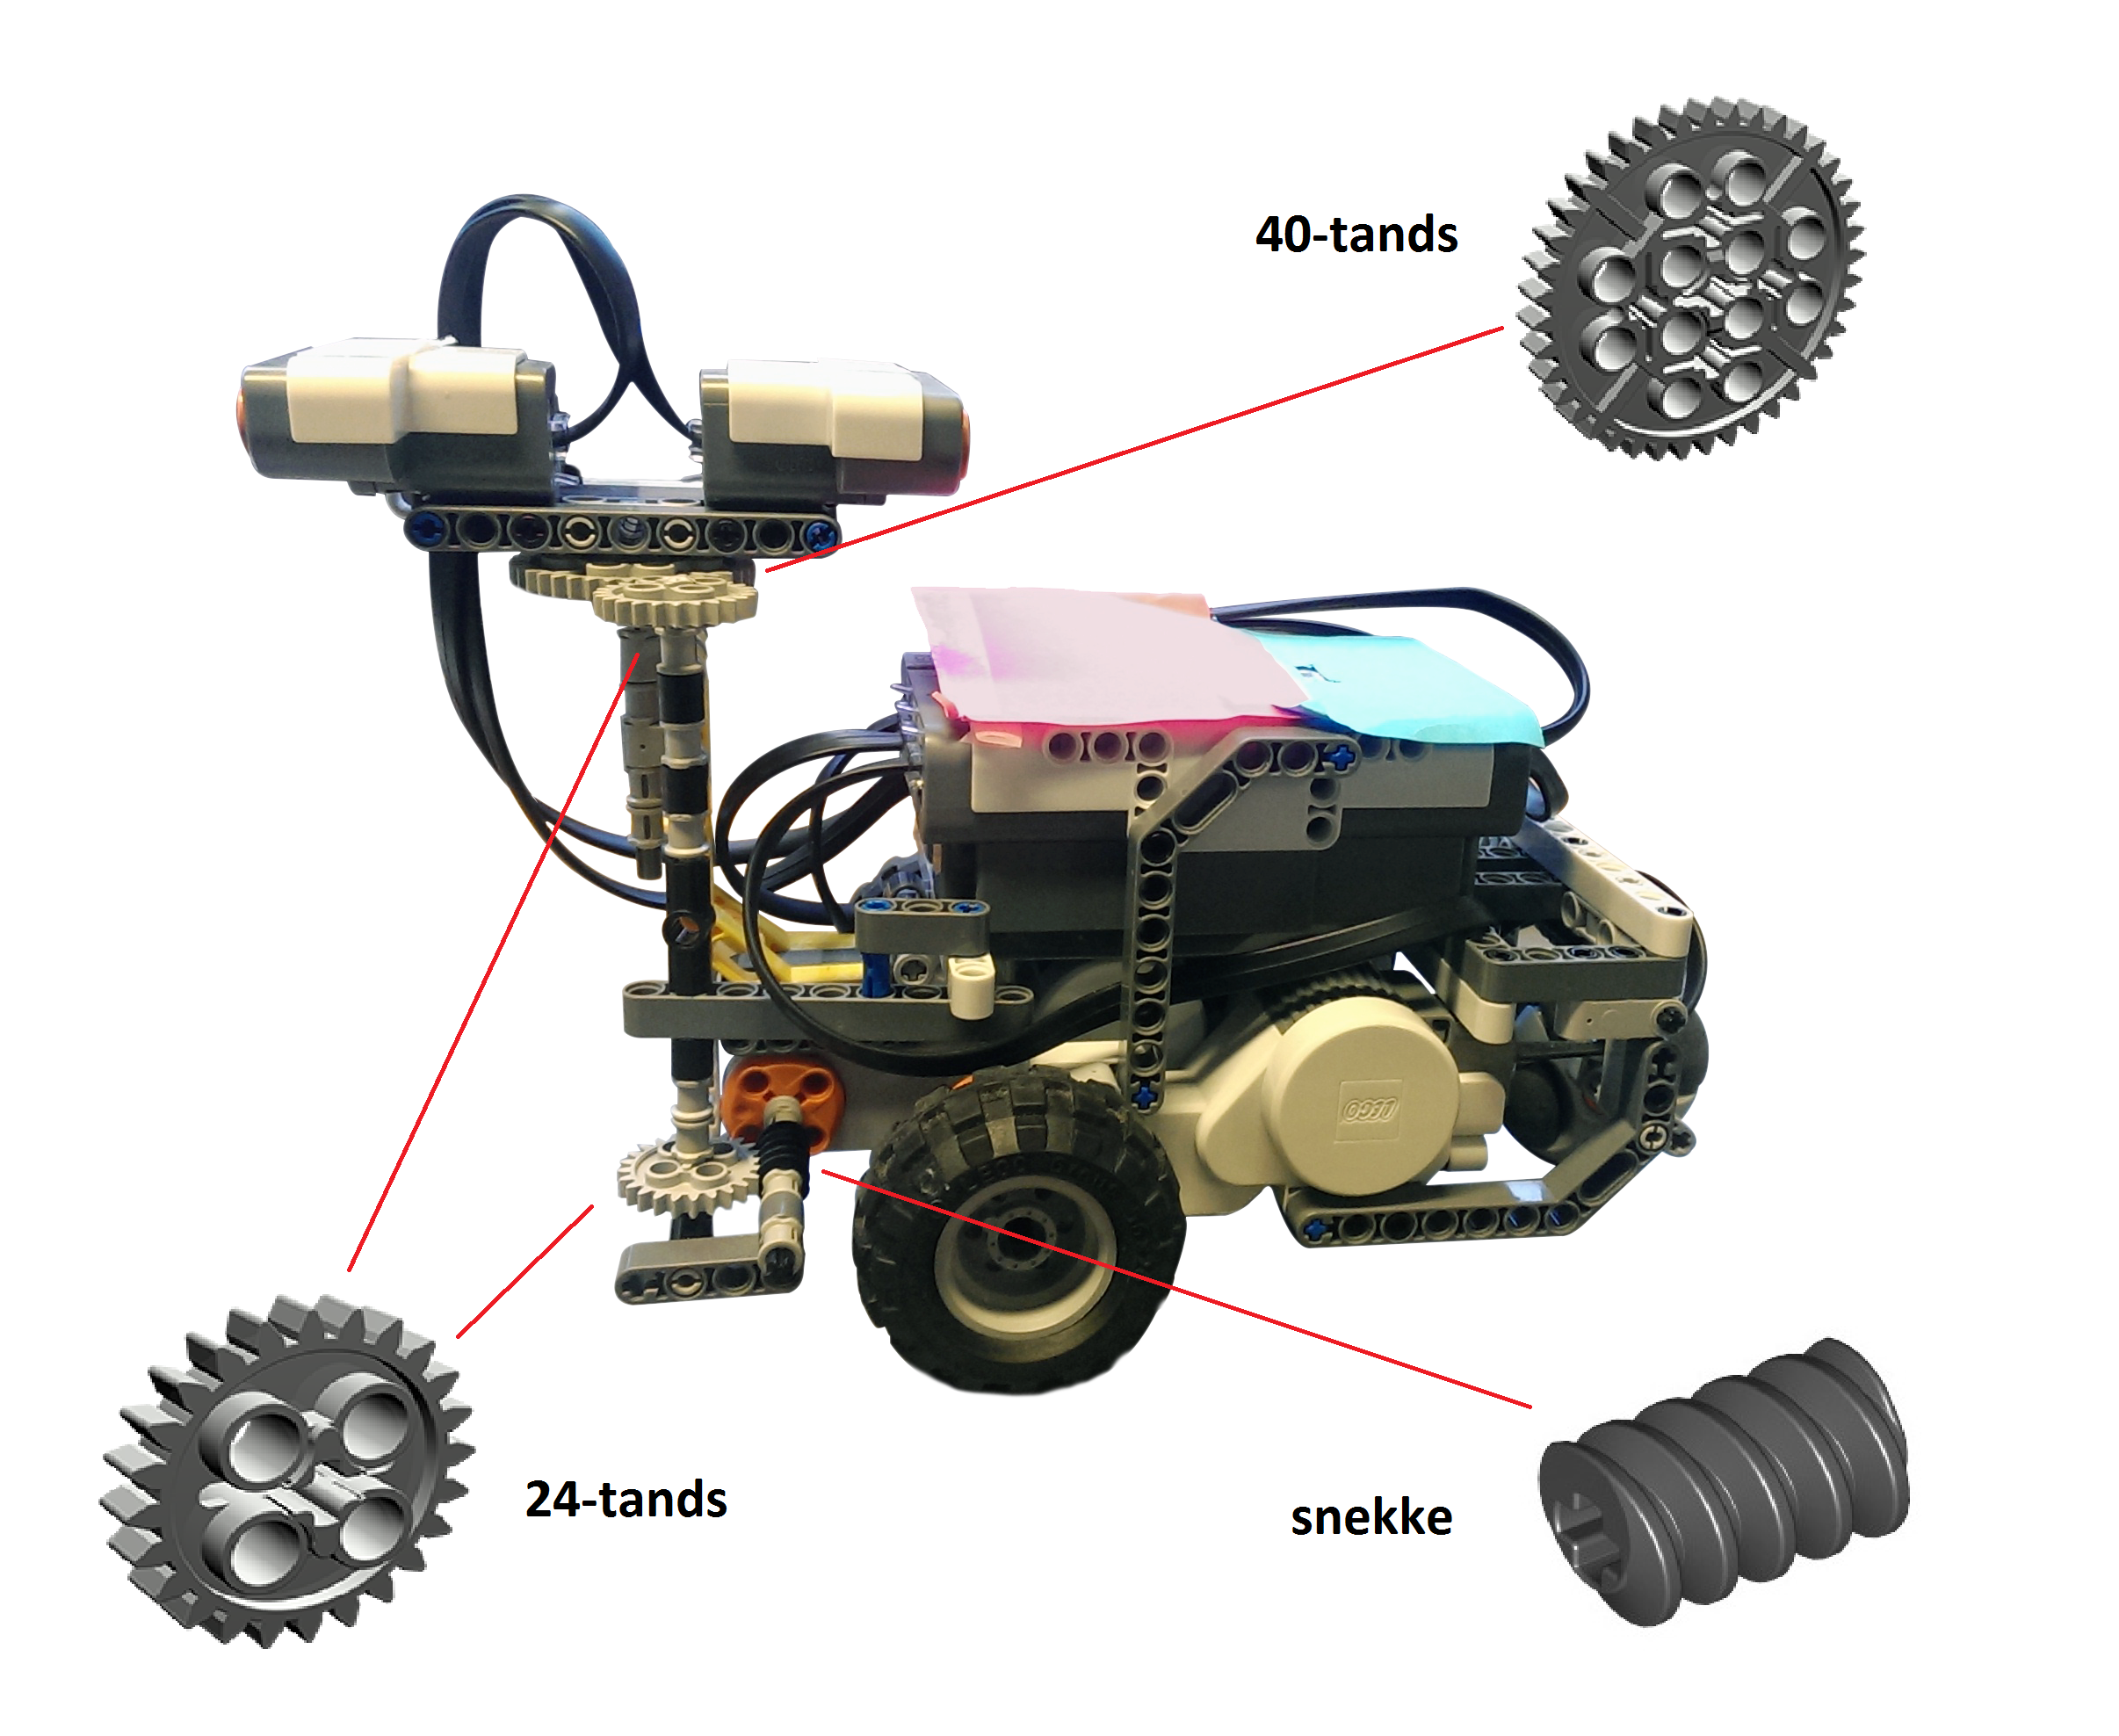
\includegraphics[scale=0.13]{whalle_with_gearing_expl}
\end{center}

\end{frame}

\subsection{Overvejelser}
\begin{frame}
\frametitle{Gearing}
\begin{itemize}
\item Gearing på hjul blev fjernet
\item Mere simpelt design
\item Unødvendigt med tårn til sensorer
\item En simplere løsning:
\begin{itemize}
\item Montere sensoren direkte på robottens krop
\item Rotere robotten når der skal måles
\end{itemize} 
\item Mindre kompleks robot design er formentlig lettere at arbejde med
\end{itemize}
\end{frame}




\section{Løsningsmetoder}
%Løsningsmetoder
\subsection{Platform}
\begin{frame}
\frametitle{Lego Mindstorms}
\begin{itemize}
\item Tilgængelighed
\item Nemt at gå til
\item Stort udvalg af sensorer
\item Mange muligheder ift. styring
\end{itemize}
\end{frame}

\begin{frame}
\frametitle{API}
\begin{itemize}
\item NXC
\begin{itemize}
\item NXC er et C-lignende sprog med gode indbyggede funktioner
\item NXC har gode indbyggede funktioner til fejlfinding
\end{itemize}
\item MindSqualls
\begin{itemize}
\item Et .NET bibliotek skrevet i C\#
\item Tillader nem direkte kommunikation med sensorer og motorer
\end{itemize}
\end{itemize}
\end{frame}
\subsection{Sensorer og Motor}
\frametitle{Valgt sensor og motor}
\begin{frame}
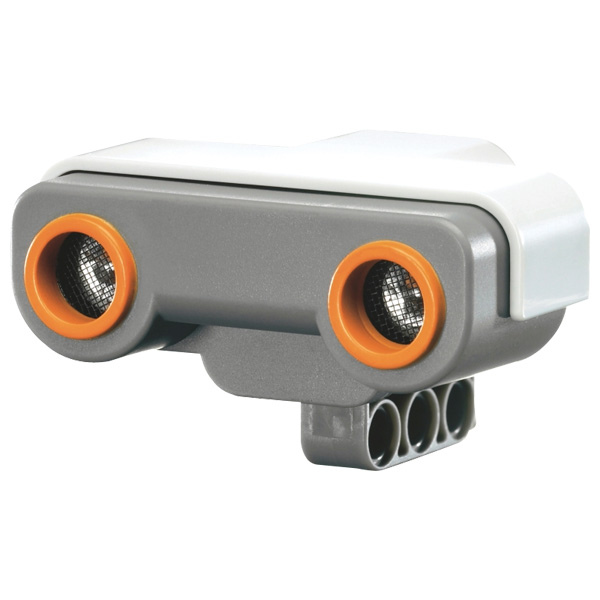
\includegraphics[width=110px, clip=true, trim = 0px 90px 0px 0px]{sensor/us}
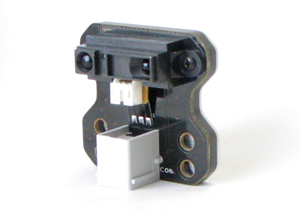
\includegraphics[width=110px]{sensor/infrared_sensor}
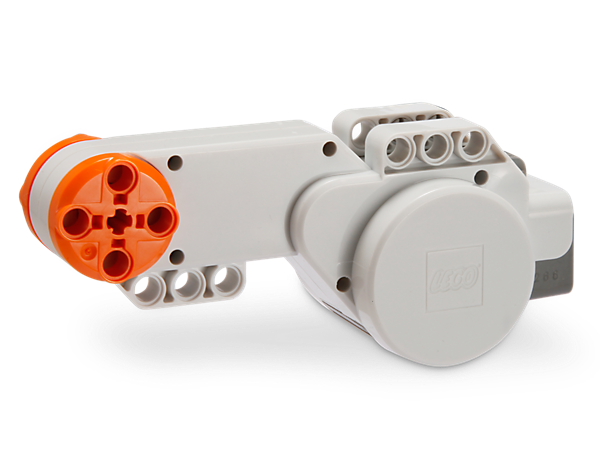
\includegraphics[width=110px]{sensor/lego_motor}
\end{frame}
\subsection{Lokalisering}
\begin{frame}
\frametitle{Valg af Kinect}
\begin{itemize}
\item Nem tilslutning til PC
\item Mange sensorer
\item Gode udviklingsværktøjer
\item Tilgængelig gennem universitetet
\end{itemize}
\end{frame}
\subsection{Mapping}
\begin{frame}
\frametitle{Occupancy grid}
\begin{itemize}
\item Til at kortlægge har vi valgt at bruge \textit{occupancy grid} algoritmen
\item \textit{Occupancy grid} er en familie af algoritmer som gør det muligt at generere konsistente kort
\item \textit{Occupancy grid} opdeler kortet i celler og tildeler en binær tilfældig variabel til hver celle
\end{itemize}
\end{frame}
\end{document}